\section{Classification}\label{5-classification}
This section describes how we developed our interface for classifying documents. First, we will first give a short of the classification part of the application. Next, we discuss how classifiers are defined. Then we will discuss how classifiers are created or loaded in the application. Finally we will discuss the interface that accepts documents and returns a prediction of the category or categories associated with the supplied document.

\subsection{Overview}
In figure \ref{fig:classify-uml} we give a concise overview of the classification subsystem. The UrbanSearch API is used to classify documents by loading an instance of the \texttt{ClassifyText} class on startup. Furthermore the API offers the possibility to create new (default) classifiers or to modify existing classifiers.\\
The \texttt{ClassifyText} object uses an implementation of the \texttt{ModelManager} class to predict categories of documents.
\begin{figure}[H]
\centering
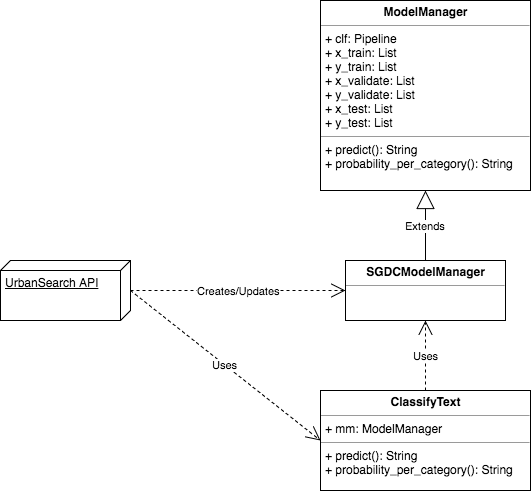
\includegraphics[width=0.6\textwidth]{classify-uml}
\caption{Diagram depicting the interaction between the API and the classification subsystems}
\label{fig:classify-uml}
\end{figure}


\subsection{Scikit Pipelines}
As explained in section \ref{sec:classification-design} we decided to use the Scikit-Learn library for all our classification functionalities. A key concept of Scikit is the so called \texttt{Pipeline}. A \texttt{Pipeline} in Scikit is an assembly of intermediate transform steps, combined with a final estimator \footnote{\url{http://scikit-learn.org/stable/modules/generated/sklearn.pipeline.Pipeline.html}}. The intermediate transforms the input data to get the best perfomance out of the final estimator. In listing \ref{lst:sdgc} we show an example of a \texttt{Pipeline} that we use in the system.\\

\begin{lstlisting}[language=python, caption={SGDC Pipeline}, label={lst:sdgc}]
sgdc = Pipeline([
            ('tfidf', TfidfVectorizer(stop_words=sw.words('dutch'))),
            ('select', SelectPercentile(f_classif)),
            ('clf', SGDClassifier(alpha=0.0001,
                                  average=False,
                                  class_weight=None,
                                  epsilon=0.1,
                                  eta0=0.0,
                                  fit_intercept=True,
                                  l1_ratio=0.15,
                                  learning_rate='optimal',
                                  loss='log',
                                  n_iter=5,
                                  n_jobs=1,
                                  penalty='l2',
                                  power_t=0.5,
                                  random_state=None,
                                  shuffle=True,
                                  verbose=0,
                                  warm_start=False))
        ])
\end{lstlisting}
This \texttt{Pipeline} consists of three parts. The "tfidf"-part transforms a text into a matrix of words with corresponding TF-IDF scores (which are calculated first using the training set). The "select"-part selects the top 10 percent of features which were returned by the previous transform, in our case the \texttt{TfidfVectorizer} transform. For this particular \texttt{Pipeline} this means that 10 percent of the features with the highest TF-IDF score are returned. Finally, the "clf"-part is the final estimator. For this \texttt{Pipeline} it is a SVM (see \ref{sec:classification-design}) that uses tochastic gradient descent (SGD) training \cite{bottou2010large}. Gradient descent tries to find the minimum of a cost function by traversing the function in the opposite way of the descent and does this step by step. SGD takes random (stochastic) steps which works more efficient when dealing with large data sets.
The fully defined pipeline can now be used to train the classifier. This is done by inputting a set of data with corresponding expected outputs.

\subsection{ModelManagers}
To provide an easy way to work with Scikit \texttt{Pipeline}s, we implemented a utility class called \texttt{ModelManager}. The \texttt{ModelManager} is a super class that should be used to implement algorithm specific \texttt{Pipeline}s, while providing easy to use interfaces for loading, saving, training and predicting. Listing \ref{lst:modman} shows a snippet of the \texttt{ModelManager} base class.

\begin{lstlisting}[language=python, caption={ModelManager base class}, label={lst:modman}]
class ModelManager(object):
    """
    ModelManager base class.
    Should only be used to load saved models from disk.
    If a file name is passed this file will be used to load a pickled
    classifier from that location on disk.
    """

    def __init__(self, filename=None):
        super(ModelManager, self).__init__()
        self.x_train = []
        self.y_train = []
        self.x_validate = []
        self.y_validate = []
        self.x_test = []
        self.y_test = []

        self.clf = self.load(filename) if filename else None

    def load(self, filename):
        """
        Load the classifier from the supplied file

        :param filename: the file containing the pickled classifier instance
        :return: a Scikit classifier object
        """
        with open(os.path.join(MODELS_DIRECTORY, filename), 'rb') as f:
            return pickle.load(f)
\end{lstlisting}

The base class can be used to implement specific \texttt{ModelManager}s which define a \texttt{Pipeline} with a final estimator of choice, like the \texttt{MultinomialNB} (Multinomial Naive Bayes) estimator used in listing \ref{lst:mnbmm}.\\

\begin{lstlisting}[language=python, caption={ModelManager using the Multinomial Naive Bayes estimator}, label={lst:mnbmm}]
class MNBModelManager(ModelManager):
    """
    An implementation of the ModelManager base class which uses a Multinomial
    Naive Bayes classifier as its default classifier.
    """

    def __init__(self, filename=None):
        super().__init__(filename)

        if not filename:
            self.clf = Pipeline([
                ('tfidf', TfidfVectorizer(stop_words=sw.words('dutch'))),
                ('anova', SelectPercentile(f_classif)),
                ('clf', MultinomialNB())
            ])
\end{lstlisting}

The \texttt{MNBModelManager} inherits all the load, save, predict and train functionality of the base class.\\
The base class can be used to load saved classifiers from disk. This is done by providing the \texttt{ModelManager} class with a file name on initialisation. If the file is found, the classifier is loaded from disk and ready to be used.

\subsection{ClassifyText Interface}
Most of the time we do not want to be busy creating and training classifiers, we want to classify documents. To provide an interface that can be used easily to input documents and get back predictions of which category a document belongs to, we implemented the \texttt{ClassifyText} class. The class loads a default classifier that should be available in the provided directory. After the class is initialised, the \texttt{predict} and \texttt{probability\_per\_category} methods can be used to predict categories for given documents.\\

The predict method, which is shown in listing \ref{lst:ct-predict}, takes a document as input and returns a prediction of the category which the inputted document best matches.\\

\begin{lstlisting}[language=python, caption={Predict method of the ClassifyText class}, label={lst:ct-predict}]
def predict(self, text, pre_processor=None):
    """
    Predict the class of the supplied text

    :param :text the text that needs to be classified
    :return: a prediction of the category for the passed text
    """
    if pre_processor:
        text = pre_processor(text)

    return self.mm.predict([text])
\end{lstlisting}



\begin{lstlisting}[language=python, caption={probability\_per\_category method of the ClassifyText class}, label={lst:ct-prob}]
def probability_per_category(self, text, pre_processor=None):
    """
    Predict the class of the supplied text

    :param :text the text that needs to be classified
    :return: a prediction of the category for the passed text
    """
    if pre_processor:
        text = pre_processor(text)

    return dict(zip(self.mm.clf.classes_,
                    self.mm.probabilities([text])[0]))
\end{lstlisting}